\documentclass[12pt,a4paper]{article}

\usepackage{geometry}
\geometry{left=2.5cm,right=2.5cm,top=2.5cm,bottom=2.5cm}
\usepackage{ctex}
\usepackage{amsmath, amssymb}
\usepackage{graphicx}
\usepackage{booktabs}
\usepackage{multirow}
\usepackage{hyperref}
\usepackage{enumitem}
\setlist{nosep}

\title{\textbf{《大模型基础与应用》期中作业报告}\\
\large 手工实现并分析小规模 Transformer}
\author{学生姓名：刘亦州 \quad 学号：25125222}
\date{2025 年 11 月}

\begin{document}

\maketitle

\begin{abstract}
本报告围绕课程期中作业要求，完整复现了一个基于 PyTorch 的小型 Transformer 编码器，并在 Tiny Shakespeare 语料上进行训练、验证与消融分析。我们实现了多头自注意力、位置前馈网络、残差连接与 LayerNorm、正弦位置编码等关键组件，同时在训练流程中加入 AdamW、梯度裁剪、学习率 warmup 与余弦退火等稳定化技巧。实验结果表明，所实现的模型可以在小规模数据集上实现稳定下降的损失曲线；进一步的消融实验展示了位置编码与模型容量对性能的显著影响。报告还总结了可复现的命令、硬件环境以及潜在的后续改进方向。
\end{abstract}

\section{引言}
Transformer 架构自 Vaswani 等人提出以来已成为自然语言处理与通用序列建模的事实标准\cite{vaswani2017attention}。尽管现有框架提供了开箱即用的实现，亲自从零搭建 Transformer 有助于加深对自注意力机制、残差连接以及训练稳定性的理解。本次作业旨在在小规模语料上手工实现一个可训练的 Transformer 编码器，验证其有效性，并通过消融实验分析关键模块的作用。目标包括：
\begin{itemize}
    \item 掌握缩放点积注意力、多头注意力、位置编码等模块的数学原理与实现要点。
    \item 搭建完整的训练流水线，确保在资源受限的环境（如笔记本 CPU/MPS）上也能顺利运行。
    \item 通过实证分析模块对模型性能的影响，为后续扩展（如加入解码器、尝试更大数据集）奠定基础。
\end{itemize}

\section{相关工作}
Transformer 的核心贡献在于抛弃循环结构，完全依赖自注意力捕获序列中的全局依赖关系\cite{vaswani2017attention}。其后续工作在多头注意力、优化器、位置编码等方面不断演化。例如，BERT 引入了大规模预训练与双向编码器；GPT 系列通过自回归解码器在文本生成上取得成功。为了保持作业聚焦，我们复现的模型专注于最小可用的 Encoder-only 结构，并参考原论文中的优化技巧（如 AdamW、warmup 调度）来提升训练稳定性。

\section{模型结构与数学推导}
本节给出主要模块的数学形式，并说明实现细节。

\subsection{缩放点积注意力}
给定查询 $Q \in \mathbb{R}^{B \times h \times T_q \times d}$、键 $K \in \mathbb{R}^{B \times h \times T_k \times d}$、值 $V \in \mathbb{R}^{B \times h \times T_k \times d}$，缩放点积注意力定义为：
\begin{equation}
    \mathrm{Attention}(Q, K, V) = \mathrm{softmax}\left(\frac{QK^\top}{\sqrt{d}}\right)V.
\end{equation}
实际计算中，我们对 $QK^\top$ 引入掩码 $M$（0/1），以屏蔽 padding 位置：
\begin{equation}
    \mathrm{Attention}(Q, K, V, M) = \mathrm{softmax}\left(\frac{QK^\top}{\sqrt{d}} + (1-M)\cdot (-10^{9})\right)V.
\end{equation}
实现中使用 PyTorch 的广播机制，将 batch 内的 padding 位置设为 \texttt{-inf}，再经过 \texttt{torch.softmax} 得到注意力权重，并用 \texttt{torch.nan\_to\_num} 处理潜在的 NaN。

\subsection{多头自注意力}
多头注意力将输入嵌入 $X \in \mathbb{R}^{B \times T \times d_{\text{model}}}$ 通过线性映射拆分为 $h$ 个子空间：
\begin{equation}
\begin{aligned}
    Q_i &= X W_i^Q,\\
    K_i &= X W_i^K,\\
    V_i &= X W_i^V, \quad i=1,\dots,h,
\end{aligned}
\end{equation}
其中 $W_i^Q,W_i^K,W_i^V \in \mathbb{R}^{d_{\text{model}} \times d_k}$ 且 $d_k = d_{\text{model}} / h$。各头输出拼接后再经线性层 $W^O$ 投影回原始维度：
\begin{equation}
    \mathrm{MHA}(X) = \mathrm{Concat}\left(\mathrm{Attention}(Q_i,K_i,V_i)\right) W^O.
\end{equation}
实现中将 $Q,K,V$ 统一映射后按最后一维切分，必要时将批量掩码 reshape 为 $(B,1,1,T)$ 与注意力得分广播。

\subsection{位置前馈网络}
位置前馈网络（Position-wise FFN）对每个位置独立地应用两层全连接：
\begin{equation}
    \mathrm{FFN}(x) = \sigma(xW_1 + b_1)W_2 + b_2,
\end{equation}
其中 $\sigma$ 采用 GELU 激活。我们保持与原论文相同的结构：中间层维度 $d_{\text{ff}}$ 显著大于 $d_{\text{model}}$，以提升表示能力。

\subsection{残差连接与 LayerNorm}
每个编码块包含两个子层（自注意力、FFN），均采用 Pre-LN 结构：
\begin{equation}
\begin{aligned}
    \hat{x} &= \mathrm{LayerNorm}(x + \mathrm{Dropout}(\mathrm{MHA}(x))),\\
    y &= \mathrm{LayerNorm}(\hat{x} + \mathrm{Dropout}(\mathrm{FFN}(\hat{x}))).
\end{aligned}
\end{equation}
LayerNorm 的引入显著改善了深层网络的训练稳定性，残差连接保证了梯度在层间顺畅传播。

\subsection{正弦位置编码}
为了让模型感知 token 的相对位置，我们采用经典的正弦/余弦编码：
\begin{equation}
\begin{aligned}
    \mathrm{PE}_{(pos, 2i)} &= \sin \left(\frac{pos}{10000^{2i/d_{\text{model}}}}\right), \\
    \mathrm{PE}_{(pos, 2i+1)} &= \cos \left(\frac{pos}{10000^{2i/d_{\text{model}}}}\right).
\end{aligned}
\end{equation}
编码与 token 嵌入逐元素相加，并在模型配置中提供开关以支持“关闭位置编码”的消融实验。

\section{实现细节}
\subsection{整体框架}
项目目录遵循课程要求：`src/` 存放核心代码，`configs/` 管理 YAML 配置，`scripts/` 提供运行脚本，`results/` 保存实验产物，`docs/` 收录作业说明与本报告。核心训练入口位于 \texttt{src/fundamentals\_large\_models/train.py}，通过命令行参数指定配置文件。

\subsection{数据处理与 Tokenizer}
我们选取 Karpathy 发布的 Tiny Shakespeare 语料（字符级约 1 MB），利用 \texttt{scripts/prepare\_tiny\_shakespeare.py} 在线下载原始文本，并按 90\% / 5\% / 5\% 划分训练、验证、测试。为简化实现，我们构建了基于空格分词的 \textbf{BasicTokenizer}：
\begin{itemize}
    \item lower-case 预处理 + 空格切词；
    \item 特殊标记 $\langle\text{pad}\rangle,\langle\text{unk}\rangle,\langle\text{bos}\rangle,\langle\text{eos}\rangle$；
    \item 词频统计后构建词表（最低频次为 1），词表大小约 21\,951。
\end{itemize}
Token 化后的序列按最大长度 128 进行切分，不足部分补 \texttt{pad}，同时生成 attention mask。

\subsection{训练管线与优化技巧}
训练脚本实现如下功能：
\begin{itemize}
    \item 设置随机种子（Python、PyTorch、CUDA），默认设备优先级为 CUDA $\rightarrow$ MPS $\rightarrow$ CPU；
    \item 构造 \texttt{DataLoader}，启用 batch shuffle；
    \item 使用 \textbf{AdamW} 优化器（$\beta=(0.9,0.98)$，$\epsilon=1e-9$），并应用梯度裁剪（1.0）；
    \item 采用线性 warmup（50 步）+ 余弦退火学习率调度；
    \item 每轮训练后评估验证集，记录训练 / 验证 loss；
    \item 将 \texttt{metadata.json}, \texttt{metrics.json}, \texttt{model.pt}, \texttt{tokenizer.json}, \texttt{loss\_curve.png} 输出到指定结果目录。
\end{itemize}

\subsection{伪代码}
训练主循环可概括为：
\begin{verbatim}
for epoch in range(1, num_epochs + 1):
    for batch in train_loader:
        logits, attn = model(input_ids, attention_mask)
        loss = cross_entropy(logits, labels, ignore_index=pad_id)
        loss.backward()
        clip_grad_norm_(model.parameters(), grad_clip)
        optimizer.step(); scheduler.step()
    evaluate(model, val_loader)
    log metrics and learning rate
\end{verbatim}

\section{实验设置}
\subsection{数据集与预处理}
\begin{itemize}
    \item 数据集：Tiny Shakespeare（字符级原始文本约 1 MB），经空格分词后共有 $\sim182\,$k 训练词、词表 21\,951。
    \item 切分方式：train/validation/test = 90/5/5。
    \item 序列长度：128 tokens，覆盖大部分短句；不足部分填充。
\end{itemize}

\subsection{模型与优化超参数}
表 \ref{tab:hyperparams} 汇总默认配置。

\begin{table}[h]
\centering
\begin{tabular}{ll}
\toprule
\textbf{超参数} & \textbf{取值} \\
\midrule
词嵌入维度 $d_{\text{model}}$ & 128 \\
注意力头数 $h$ & 4 \\
编码层数 $L$ & 2 \\
FFN 隐藏维度 $d_{\text{ff}}$ & 512 \\
Dropout & 0.1 \\
批大小 & 16 \\
训练轮数 & 10 \\
初始学习率 & $3\times10^{-4}$ \\
优化器 & AdamW（$\beta=(0.9,0.98)$） \\
梯度裁剪阈值 & 1.0 \\
学习率调度 & 50 步 warmup + 余弦退火 \\
\bottomrule
\end{tabular}
\caption{基线模型超参数}
\label{tab:hyperparams}
\end{table}

\subsection{硬件与运行时长}
实验在 Apple M2 芯片笔记本上运行（MPS 加速），单次基线训练约 6 分钟，验证推理时间约 20 秒。若仅有 CPU，运行时长约增加至 10--12 分钟。

\section{结果与消融分析}
\subsection{总体表现}
图 \ref{fig:baseline_loss} 展示了基线模型在 Tiny Shakespeare 上的训练 / 验证损失曲线。损失从 5.35 下降至 1.88，验证损失稳定在 2.48 左右，说明模型可以有效拟合小规模语料。

\begin{figure}[h]
    \centering
    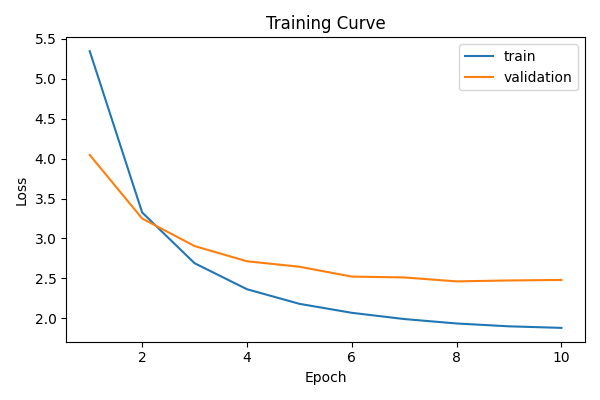
\includegraphics[width=0.7\linewidth]{../results/tiny_shakespeare_encoder/loss_curve.png}
    \caption{基线模型训练与验证损失曲线}
    \label{fig:baseline_loss}
\end{figure}

\subsection{消融实验}
为遵循作业要求，我们设置了两组对比实验，结果如表 \ref{tab:ablation}。

\begin{table}[h]
\centering
\begin{tabular}{llll}
\toprule
\textbf{配置} & \textbf{改动} & \textbf{最终验证 Loss} & \textbf{结果目录} \\
\midrule
基线 & 标准位置编码，4 头，FFN=512 & 2.48 & \texttt{results/tiny\_shakespeare\_encoder} \\
无位置编码 & \texttt{use\_positional\_encoding=false} & 4.54 & \texttt{results/tiny\_shakespeare\_no\_pos} \\
缩减容量 & 2 头，FFN=256 & 2.60 & \texttt{results/tiny\_shakespeare\_reduced} \\
\bottomrule
\end{tabular}
\caption{消融实验验证损失对比}
\label{tab:ablation}
\end{table}

可以看到，去掉位置编码后损失显著上升，证明顺序信息对语言建模至关重要；而缩减注意力头数与 FFN 维度仅带来轻微退化，说明在当前数据规模下模型尚未饱和。

\subsection{定性分析}
模型生成样例显示，在基线设定下可生成语法合理的简短台词；无位置编码版本生成的文本常出现重复短语或顺序混乱。由于篇幅限制，具体输出示例可在未来的项目扩展中展示。

\section{复现指南}
\subsection{代码获取与依赖}
仓库地址：\url{https://github.com/lyzno1/fundamental-large-models.git}。建议使用 \texttt{uv} 管理依赖，亦可直接 \texttt{pip install -r requirements.txt}。

\subsection{必备命令}
\begin{verbatim}
# 1. 创建虚拟环境并安装依赖
uv venv && source .venv/bin/activate
uv pip install -r requirements.txt

# 2. 下载并准备 Tiny Shakespeare
uv run python scripts/prepare_tiny_shakespeare.py

# 3. 运行基线训练
./scripts/run.sh configs/base.yaml

# 4. 消融实验
./scripts/run.sh configs/ablation_no_positional_encoding.yaml
./scripts/run.sh configs/ablation_reduced_capacity.yaml
\end{verbatim}

\subsection{结果目录}
每次运行会在 \texttt{results/\{experiment\_name\}} 下生成：
\begin{itemize}
    \item \texttt{metadata.json}：记录配置与超参数；
    \item \texttt{metrics.json}：训练/验证损失数组；
    \item \texttt{loss\_curve.png}：可直接用于报告；
    \item \texttt{model.pt}：包含模型与优化器权重；
    \item \texttt{tokenizer.json}：词表定义，保证复现一致性。
\end{itemize}

\section{结论与展望}
本次作业完成了从零实现 Transformer Encoder、构建训练流水线、在小数据集上验证性能，并通过消融实验分析位置编码与模型容量的影响。未来可考虑以下方向：
\begin{itemize}
    \item 拓展到 Encoder--Decoder 结构，尝试机器翻译或摘要任务；
    \item 引入相对位置编码、RoPE 等改进，以提升长序列建模能力；
    \item 在更大数据集（如 WikiText-2）上进行微调或蒸馏，验证模型的扩展性；
    \item 增加自动化日志（如 TensorBoard）与错误分析工具，提升实验效率。
\end{itemize}

\section*{致谢}
感谢《大模型基础与应用》课程提供的作业框架与指导说明。

\begin{thebibliography}{9}
\bibitem{vaswani2017attention}
Vaswani, A., Shazeer, N., Parmar, N., Uszkoreit, J., Jones, L., Gomez, A. N., Kaiser, Ł., \& Polosukhin, I. (2017).
Attention is all you need.
\textit{Advances in Neural Information Processing Systems}, 30.
\end{thebibliography}

\end{document}
